\documentclass[conference]{IEEEtran}
\IEEEoverridecommandlockouts
% The preceding line is only needed to identify funding in the first footnote. If that is unneeded, please comment it out.
\usepackage[utf8]{inputenc}
\usepackage[vietnamese]{babel}
\usepackage{amsmath}
\usepackage{cite}
\usepackage{amsmath,amssymb,amsfonts}
\usepackage{algorithmic}
\usepackage{graphicx}
\usepackage{textcomp} 
\usepackage{xcolor}
\usepackage{biblatex}
\addbibresource{ref.bib}
\usepackage{fancyhdr}
\usepackage{adjustbox}
\usepackage{lipsum}
\usepackage{tabularx} % for better control over table width
\usepackage{multirow} % Thêm package multirow
\usepackage{array}
\usepackage{makecell}
\pagestyle{fancy}
\usepackage{xcolor}
\usepackage{float}
\usepackage{relsize}
\usepackage{caption}
\captionsetup[table]{skip=10pt} 
\captionsetup[table]{belowskip=-20pt} % Khoảng cách giữa bảng và văn bản tiếp theo

\fancyhf{}
\rfoot{\thepage}
\def\BibTeX{{\rm B\kern-.05em{\sc i\kern-.025em b}\kern-.08em
    T\kern-.1667em\lower.7ex\hbox{E}\kern-.125emX}}
\begin{document}

\title{DỰ BÁO GIÁ KIM LOẠI QUÝ SỬ DỤNG CÁC MÔ HÌNH THỐNG KÊ, HỌC MÁY VÀ HỌC SÂU\\
}

\author{\IEEEauthorblockN{1. Phan Minh Trí}
\IEEEauthorblockA{\textit{Khoa Hệ thống Thông tin} \\
\textit{Trường Đại học Công nghệ Thông tin}\\
21522709@gm.uit.edu.vn}
\and
\IEEEauthorblockN{2. Vương Thanh Linh}
\IEEEauthorblockA{\textit{Khoa Hệ thống Thông tin} \\
\textit{Trường Đại học Công nghệ Thông tin}\\
21521082@gm.uit.edu.vn}
\and
\IEEEauthorblockN{3. Lê Nguyễn Hoàng Huy}
\IEEEauthorblockA{\textit{Khoa Hệ thống Thông tin} \\
\textit{Trường Đại học Công nghệ Thông tin}\\
21520915@gm.uit.edu.vn}
\and
\IEEEauthorblockN{4. Trần Hạnh Thảo}
\IEEEauthorblockA{\textit{Khoa Hệ thống Thông tin} \\
\textit{Trường Đại học Công nghệ Thông tin}\\
21522609@gm.uit.edu.vn}
\and
\IEEEauthorblockN{                }
\IEEEauthorblockA{\textit{                      } \\
\textit{                                  }\\
                     }
                     \and
\IEEEauthorblockN{                }
\IEEEauthorblockA{\textit{                      } \\
\textit{                                  }\\
                     }
                     \and
\IEEEauthorblockN{                }
\IEEEauthorblockA{\textit{                      } \\
\textit{                                  }\\
                     }
                     \and
\IEEEauthorblockN{                }
\IEEEauthorblockA{\textit{                      } \\
\textit{                                  }\\
                     }
                     \and
\IEEEauthorblockN{                }
\IEEEauthorblockA{\textit{                      } \\
\textit{                                  }\\
                     }
                     \and
\IEEEauthorblockN{                }
\IEEEauthorblockA{\textit{                      } \\
\textit{                                  }\\
                     }\and
\IEEEauthorblockN{                }
\IEEEauthorblockA{\textit{                      } \\
\textit{                                  }\\
                     }
\and
\IEEEauthorblockN{5. Nguyễn Thị Tường Vi}
\IEEEauthorblockA{\textit{Khoa Hệ thống Thông tin} \\
\textit{Trường Đại học Công nghệ Thông tin}\\
21522787@gm.uit.edu.vn}
}

\maketitle
\thispagestyle{fancy}
\begin{abstract}
Trên thị trường hiện nay, vàng (Gold), bạch kim (Platinum) và Palladium là các kim loại quý hiếm, có giá trị cao và nhu cầu về các kim loại này không bao giờ giảm. Xu hướng tỷ giá của kim loại quý cho thấy đây là một trong những phương án đầu tư tốt nhất hiện nay. Vì vậy, mối quan tâm đến việc sử dụng các mô hình thống kê, học máy và học sâu để hiểu rõ và dự báo xu hướng của tỷ giá này có ý nghĩa rất lớn đối với nền kinh tế đất nước. Bài báo sẽ nghiên cứu các ý tưởng dự báo tỷ giá vàng (Gold), bạch kim (Platinum) và Palladium bằng các mô hình: Linear Regression (LR), Exponential Smoothing Trend (ETS), ARIMA, Random Forest (RF), Support Vector Regression (SVR), Recurrent Neural Network (RNN), Gated Recurrent Unit  (GRU), Long Short Term Memory (LSTM), Timesnet, Autoformer. Nghiên cứu áp dụng 10 mô hình dự báo khác nhau để tìm ra mô hình nào hoạt động tốt nhất trên tập dữ liệu có sẵn. Bộ dữ liệu về giá kim loại quý được chia theo tập train:test với 3 tỷ lệ là 6:4, 7:3, 8:2. Sau đó thực hiện so sánh hiệu suất của các mô hình dựa trên ba độ đo: MSE, RMSE, MAPE. Cuối cùng, thực hiện dự báo giá của kim loại quý trong 30, 60 và 90 ngày tiếp theo đối với tất cả mô hình. Kết quả cho thấy mô hình TimesNet, RNN và GRU có hiệu suất ổn định nhất và có thể giúp cải thiện dự báo. Từ đó, đưa ra các quyết định hiệu quả trong thị trường thực tế và giúp ích cho việc phát triển và đầu tư vào các kim loại quý.
\end{abstract}

\begin{IEEEkeywords}
Dự báo, Kim loại quý, LR, ETS, ARIMA, RF, SVR, RNN, GRU, LSTM, TimesNet, Autoformer
\end{IEEEkeywords}

\section{GIỚI THIỆU}
\input{section/intro.tex}\\

\section{CƠ SỞ LÝ THUYẾT}
\input{section/relatedworks/LR.tex}

\input{section/relatedworks/ETS.tex}

\input{section/relatedworks/ARIMA.tex}

\input{section/relatedworks/RF.tex}

\begin{figure}[H]
\centerline{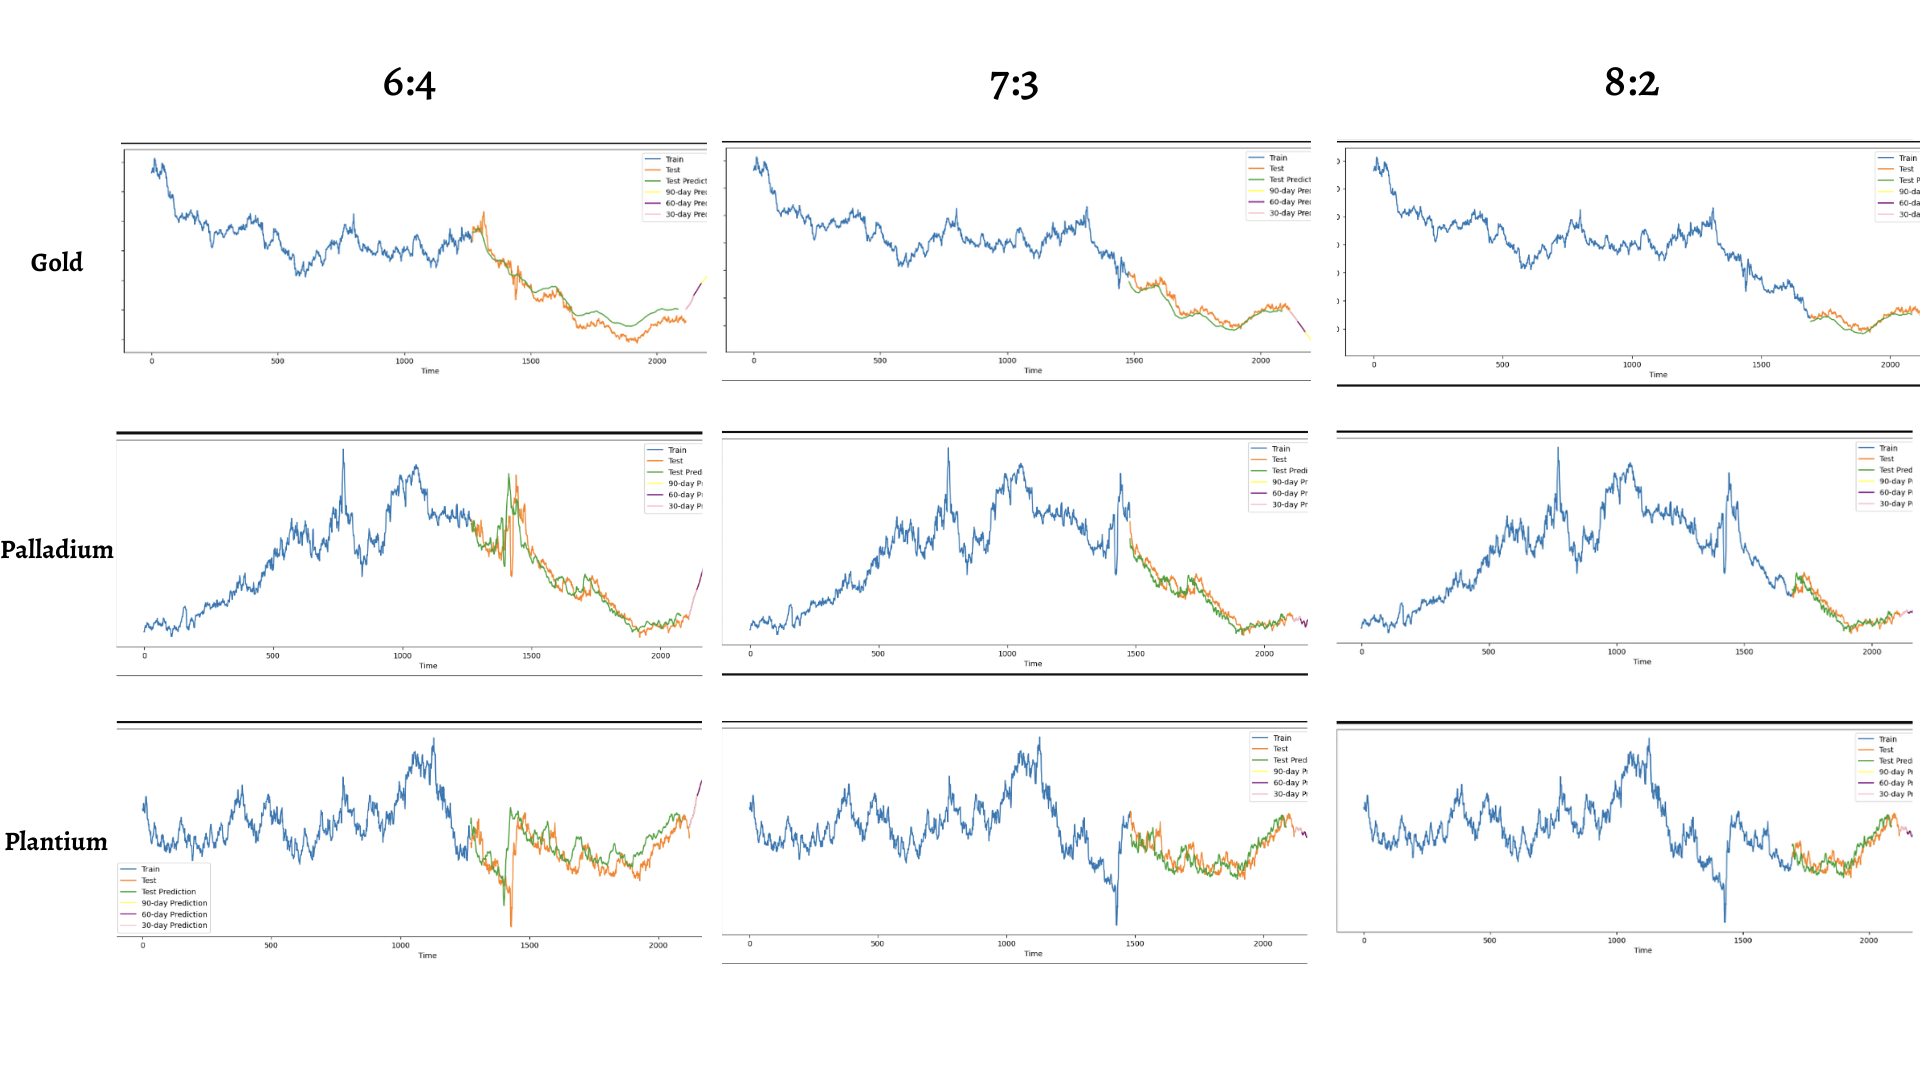
\includegraphics[width=0.45\textwidth]{img/SVR_result.png}}
\caption{Kết quả thực nghiệm SVR}
\label{fig}
\end{figure}

Recurrent Neural Network (RNN) là một mạng neural hồi quy sử dụng dữ liệu tuần tự hoặc chuỗi thời gian với 3 thành phần chính là Input layer, Hidden layer và Output layer\cite{website2}.

Điểm đặc trưng của RNN là "bộ nhớ" của chúng cho phép sử dụng các thông tin từ đầu vào trước đó để ảnh hưởng đến đầu vào và đầu ra hiện tại, khác với mạng nơ-ron truyền thống.

Trong bài toán dự đoán giá vàng, RNN sử dụng 2 lớp SimpleRNN và Dense với từng vai trò khác nhau. Lớp SimpleRNN có tác dụng trích xuất các đặc trưng của dữ liệu chuỗi thời gian để nhận diện và học các bước xu hướng thời gian trước đó. Trong khi đó lớp Dense nhận các trích xuất đặc trưng từ lớp SimpleRNN và tổng hợp thông tin tin từ các đơn vị trong lớp RNN để áp dụng các phép biến đổi tuyến tính hoặc phi tuyến. Từ đó, dưới sự kết hợp của 2 lớp, mô hình RNN có thể đưa ra dự đoán giá vàng trong tương lai một cách chính xác.
\begin{figure}[htbp]
\centerline{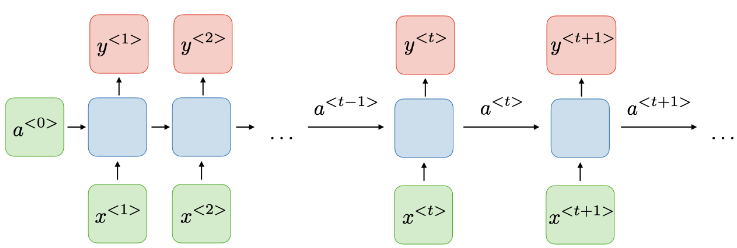
\includegraphics[width=0.4\textwidth]{img/RNN.png}}
\caption{Kiến trúc RNN}
\label{fig}
\end{figure}

RNN được biểu diễn bằng công thức sau:
\begin{align}
    a^{<t>} &= g_1(W_{aa}a^{<t-1>} + W_{ax}x^{<t>} + b_a) \\
    y^{<t>} &= g_2(W_{ya}a^{<t>} + b_y)
\end{align}

Trong đó:
\begin{itemize}
    \item $x^{<t>}$: giá trị đầu vào tại thời điểm $t$
    \item $y^{<t>}$: giá trị đầu ra tại thời điểm $t$
    \item $a^{<t>}$: giá trị kích hoạt
    \item $W_{aa}, W_{ax}, W_{ya}$: các ma trận trọng số
    \item $b_a, b_y$: vector độ lệch
    \item $g_1, g_2$: các hàm kích hoạt
\end{itemize}

\input{section/relatedworks/GRU.tex}

\input{section/relatedworks/LSTM.tex}

\input{section/relatedworks/TimesNet.tex}

\input{section/relatedworks/Autoformer.tex}\\

\section{ĐỐI TƯỢNG NGHIÊN CỨU}
\input{section/dataset.tex}
\hfill
\section{PHƯƠNG PHÁP NGHIÊN CỨU}
\subsection{Linear Regression (LR)}
\input{section/methods/LR.tex}

\subsection{Exponential Smoothing Trend (ETS)}
\input{section/methods/ETS.tex}

\subsection{ARIMA}
\input{section/methods/ARIMA.tex}

\subsection{Random Forest (RF)}
\input{section/methods/RF.tex}

\subsection{Support Vector Regression (SVR)}
SVM (Support Vector Machines) là một phương pháp máy vector hỗ trợ được sử dụng cho các bài toán phân loại. Mục tiêu của SVM là tìm một siêu phẳng (hyperplane) tốt nhất phân chia dữ liệu thành các lớp khác nhau. Tuy nhiên, trong bài toán dự đoán giá kim loại quý, cần quan tâm đến việc dự đoán một giá trị thực (giá kim loại) dựa trên đặc trưng đầu là giá đóng cửa (Close). Do đó, nhóm sử dụng SVR để tìm cách dự đoán một giá trị thực. SVR sẽ tìm một hàm hồi quy tốt nhất mà sai số của các dự đoán nằm trong khoảng chấp nhận được. SVR có thể sử dụng các hàm hạt nhân (kernel) để chuyển đổi không gian đầu vào sang không gian đặc trưng cao giúp cho việc xử lý các dữ liệu tuyến tính và phi tuyến. Một kernel tuyến tính là tích vô hướng đơn giản giữa hai vector đầu vào, trong khi một kernel phi tuyến là một hàm phức tạp hơn có thể nắm bắt các mẫu phức tạp hơn trong dữ liệu. 

Không giống như các mô hình hồi quy truyền thống, SVR tập trung vào việc giảm thiểu lỗi dự đoán thay vì khớp dữ liệu một cách chính xác. Để đạt được điều này bằng cách tìm một siêu phẳng tối ưu tối ưu hóa khoảng cách hay biên, giữa các giá trị dự đoán và các điểm dữ liệu thực tế. SVR đạt được sự cân bằng giữa tính đơn giản và tính linh hoạt bằng cách cho phép một mức đúng sai nhất định, hay biên độ lỗi, xung quanh các giá trị dự đoán.


Hàm hồi quy trong SVR:
\[
f(x) = \langle w, x \rangle + b
\]\\
Hàm mất mát E-insensitive:
\[
L(y, F(x_i, \hat{w})) = \max(0, y - F(x_i, \hat{w}) - \varepsilon)
\]\\
Trong đó:\\
    \indent\textbullet\ \(L(y,F(x_i,\hat{w})\): hàm lỗi.\\
    \indent\textbullet\ \(y\): giá trị thực.\\
    \indent\textbullet\ \(F(x_i,\hat{w})\): sai số ngẫu nhiên.\\
    \indent\textbullet\ \(\varepsilon\): tham số điều chỉnh cho phép sai lệch.\\
Dưới đây là một số hàm kernel có thể sử dụng trong SVR
\begin{table}[htbp]
  \centering
\begin{tabular}{|c|c|}
    \hline
     Kernel& Hàm\\ \hline
     Linear &  $f(X1,X2)=X1^TX2$\\ \hline
     Polynomial & $f(X1,X2)=(X1^TX2 +1)^d$ \\ \hline
     Sigmoid &  $f(X1,X2)=\tanh(\alpha x^{T}y+x)$\\ \hline
     RBF &  $f(X1,X2)=e^{\frac{-{\mid\mid x1-x2 \mid\mid}^2}{2\sigma^2}}$\\ \hline
\end{tabular}
\caption{Bảng tổng hợp các hàm kernel của SVR}
\end{table}

\hfill\\
\textbf{Linear}: Đây là kernel đơn giản nhất và cơ bản nhất trong SVR. Linear phù hợp khi dữ liệu có thể được phân tách tuyến tính trong không gian đầu vào.\\
\textbf{Polynomial}: Kernel này biến đổi dữ liệu đầu vào không gian đa thức, được xác định bởi tham số bậc và hệ số độ lệch.\\
\textbf{Sigmoid}: Kernel này biến đổi dữ liệu đầu vào thành không gian phi tuyến bằng cách sử dụng hàm sigmoid. Hàm sigmoid áp dụng phép biến đổi phi tuyến lên tích vô hướng của hai vector đầu vào. Ngoài ra có thể được sử dụng cho các bài toán có dữ liệu nhị phân.\\
\textbf{RBF}: Đây là kernel phi tuyến phổ biến và cho phép mô hình học các cấu trúc phi tuyến phức tạp. Hàm RBF được xác định bởi tham số độ dốc.

\subsection{Recurrent Neural Network (RNN)}
Recurrent Neural Network (RNN) là một mạng neural hồi quy sử dụng dữ liệu tuần tự hoặc chuỗi thời gian với 3 thành phần chính là Input layer, Hidden layer và Output layer\cite{website2}.

Điểm đặc trưng của RNN là "bộ nhớ" của chúng cho phép sử dụng các thông tin từ đầu vào trước đó để ảnh hưởng đến đầu vào và đầu ra hiện tại, khác với mạng nơ-ron truyền thống.

Trong bài toán dự đoán giá vàng, RNN sử dụng 2 lớp SimpleRNN và Dense với từng vai trò khác nhau. Lớp SimpleRNN có tác dụng trích xuất các đặc trưng của dữ liệu chuỗi thời gian để nhận diện và học các bước xu hướng thời gian trước đó. Trong khi đó lớp Dense nhận các trích xuất đặc trưng từ lớp SimpleRNN và tổng hợp thông tin tin từ các đơn vị trong lớp RNN để áp dụng các phép biến đổi tuyến tính hoặc phi tuyến. Từ đó, dưới sự kết hợp của 2 lớp, mô hình RNN có thể đưa ra dự đoán giá vàng trong tương lai một cách chính xác.
\begin{figure}[htbp]
\centerline{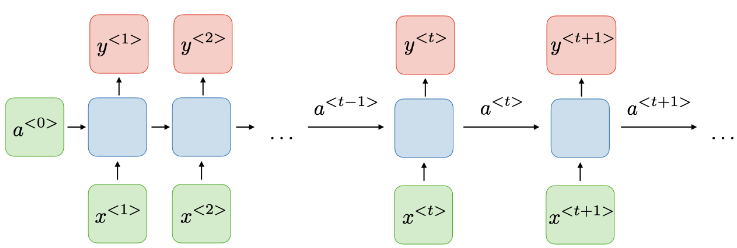
\includegraphics[width=0.4\textwidth]{img/RNN.png}}
\caption{Kiến trúc RNN}
\label{fig}
\end{figure}

RNN được biểu diễn bằng công thức sau:
\begin{align}
    a^{<t>} &= g_1(W_{aa}a^{<t-1>} + W_{ax}x^{<t>} + b_a) \\
    y^{<t>} &= g_2(W_{ya}a^{<t>} + b_y)
\end{align}

Trong đó:
\begin{itemize}
    \item $x^{<t>}$: giá trị đầu vào tại thời điểm $t$
    \item $y^{<t>}$: giá trị đầu ra tại thời điểm $t$
    \item $a^{<t>}$: giá trị kích hoạt
    \item $W_{aa}, W_{ax}, W_{ya}$: các ma trận trọng số
    \item $b_a, b_y$: vector độ lệch
    \item $g_1, g_2$: các hàm kích hoạt
\end{itemize}

\subsection{Gated Recurrent Unit (GRU)}
\input{section/methods/GRU.tex}

\subsection{Long Short Term Memory (LSTM)}
\input{section/methods/LSTM.tex}

\subsection{Autoformer}
\input{section/methods/Autoformer.tex}

\subsection{TimesNet}
\input{section/methods/TimesNet.tex}

\subsection{Độ đo}
Để đánh giá năng lực dự đoán của các mô hình sử dụng trong đồ án, nhóm sử dụng ba phép đo hiệu suất bao gồm: Mean Absolute Percentage Error (MAPE), Root Mean Square Error (RMSE) và Mean Square Error (MSE).

Độ đo MAPE đo lường sai số tuyệt đối trung bình giữa giá trị dự đoán và giá trị thực tế với công thức như sau:
\[
MAPE = \frac{\sum_{i=1}^{n}\left(\frac{abs(y_i - f_i)}{y_i}\right)}{n}
\]

Độ đo MSE tính toán trung bình bình phương của các sai số giữa giá trị thực tế và giá trị dự báo với công thức sau:
\[
MSE = \frac{\sum(f_i - y_i)^2}{N}
\]

Độ đo RMSE đo lường khoảng cách trung bình giữa các giá trị dự đoán và thực tế với công thức như sau:
\[
RMSE = \sqrt{\frac{\sum_{i=1}^{n}(f_i - y_i)^2}{n}}
\]
Trong đó:\\
    \indent\textbullet\ \(f_{i}\) là giá trị dự đoán cho mẫu thứ i.\\
    \indent\textbullet\ \(y_{i}\) là giá trị thực tế cho mẫu thứ i.\\
    \indent\textbullet\ \(N\) là số lượng mẫu.


\section{Thực nghiệm}
\input{section/results/LR.tex}

\input{section/results/ETS.tex}

\input{section/results/ARIMA.tex}

\input{section/results/RF.tex}

\begin{figure}[H]
\centerline{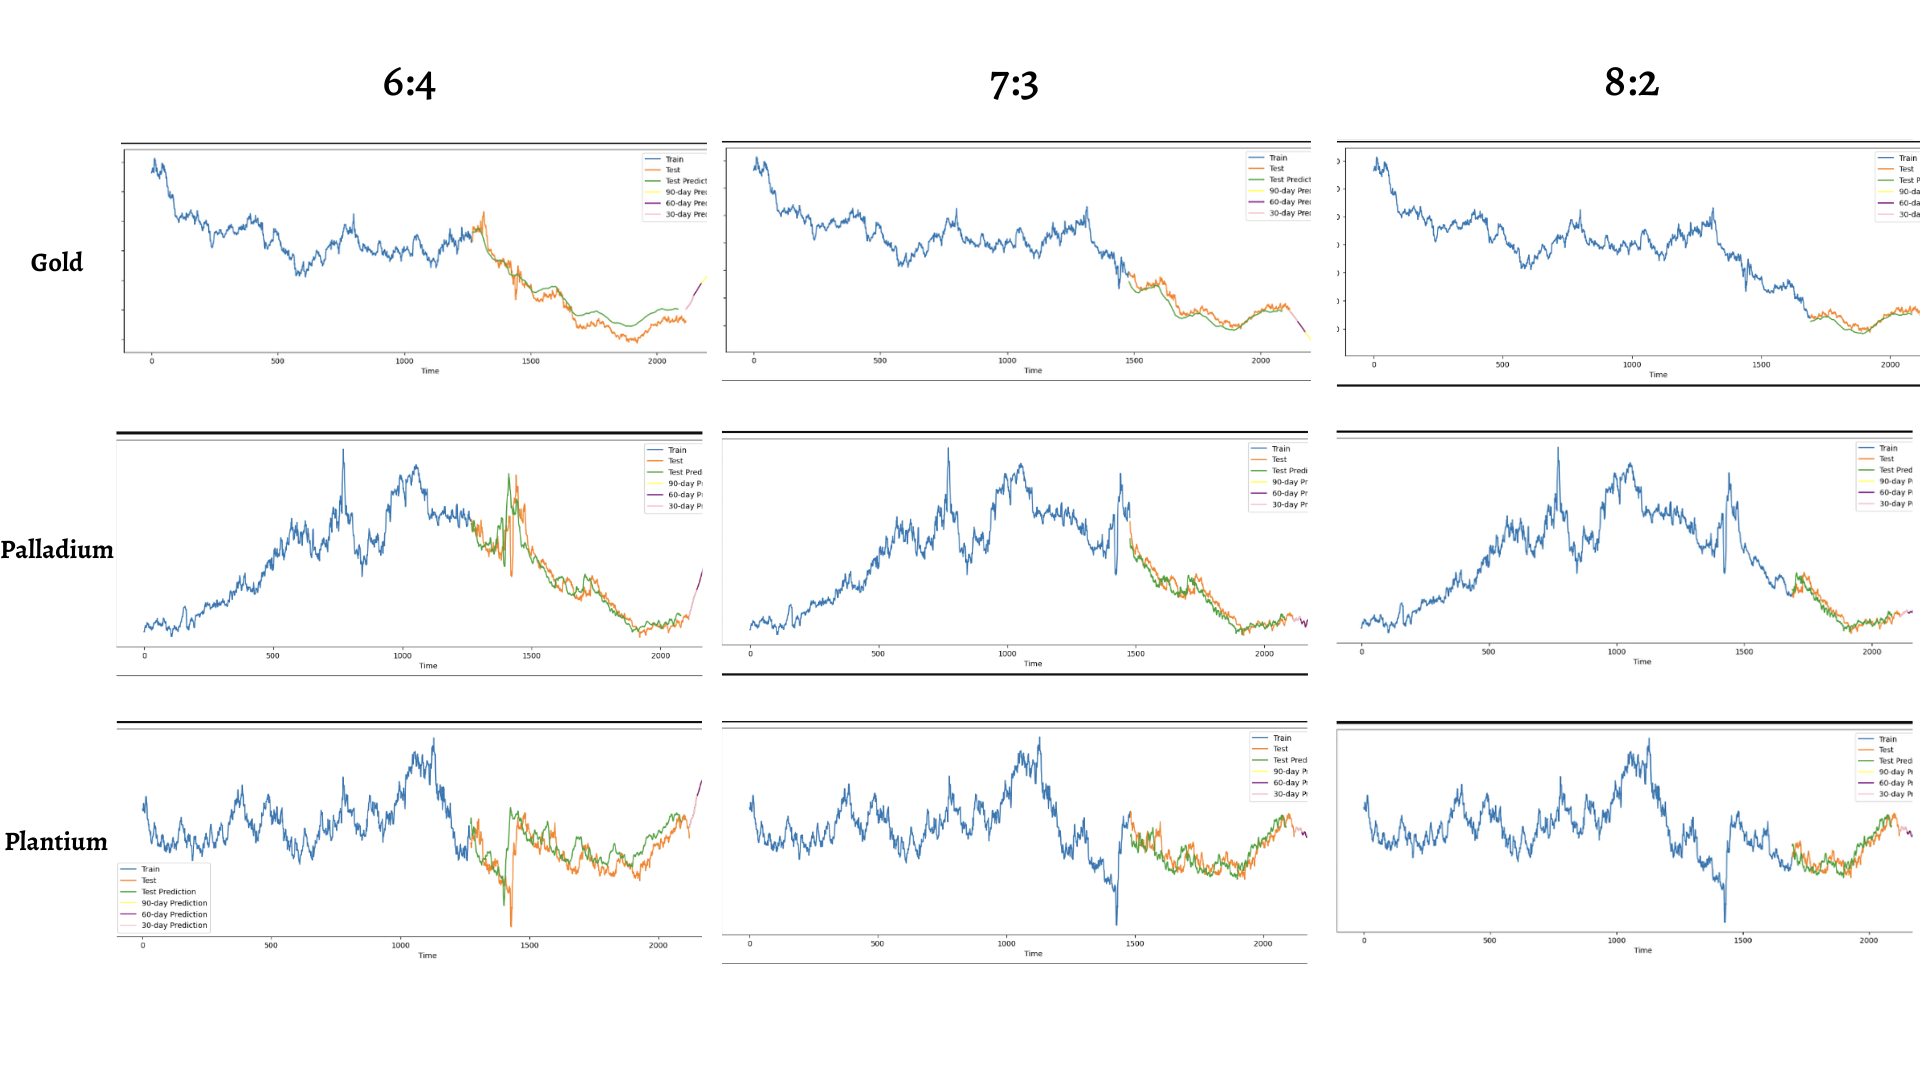
\includegraphics[width=0.45\textwidth]{img/SVR_result.png}}
\caption{Kết quả thực nghiệm SVR}
\label{fig}
\end{figure}

Recurrent Neural Network (RNN) là một mạng neural hồi quy sử dụng dữ liệu tuần tự hoặc chuỗi thời gian với 3 thành phần chính là Input layer, Hidden layer và Output layer\cite{website2}.

Điểm đặc trưng của RNN là "bộ nhớ" của chúng cho phép sử dụng các thông tin từ đầu vào trước đó để ảnh hưởng đến đầu vào và đầu ra hiện tại, khác với mạng nơ-ron truyền thống.

Trong bài toán dự đoán giá vàng, RNN sử dụng 2 lớp SimpleRNN và Dense với từng vai trò khác nhau. Lớp SimpleRNN có tác dụng trích xuất các đặc trưng của dữ liệu chuỗi thời gian để nhận diện và học các bước xu hướng thời gian trước đó. Trong khi đó lớp Dense nhận các trích xuất đặc trưng từ lớp SimpleRNN và tổng hợp thông tin tin từ các đơn vị trong lớp RNN để áp dụng các phép biến đổi tuyến tính hoặc phi tuyến. Từ đó, dưới sự kết hợp của 2 lớp, mô hình RNN có thể đưa ra dự đoán giá vàng trong tương lai một cách chính xác.
\begin{figure}[htbp]
\centerline{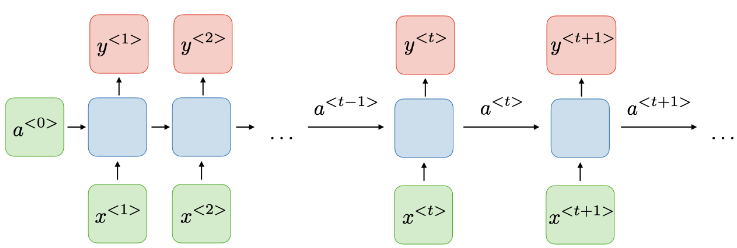
\includegraphics[width=0.4\textwidth]{img/RNN.png}}
\caption{Kiến trúc RNN}
\label{fig}
\end{figure}

RNN được biểu diễn bằng công thức sau:
\begin{align}
    a^{<t>} &= g_1(W_{aa}a^{<t-1>} + W_{ax}x^{<t>} + b_a) \\
    y^{<t>} &= g_2(W_{ya}a^{<t>} + b_y)
\end{align}

Trong đó:
\begin{itemize}
    \item $x^{<t>}$: giá trị đầu vào tại thời điểm $t$
    \item $y^{<t>}$: giá trị đầu ra tại thời điểm $t$
    \item $a^{<t>}$: giá trị kích hoạt
    \item $W_{aa}, W_{ax}, W_{ya}$: các ma trận trọng số
    \item $b_a, b_y$: vector độ lệch
    \item $g_1, g_2$: các hàm kích hoạt
\end{itemize}

\input{section/results/GRU.tex}

\input{section/results/LSTM.tex}

\input{section/results/TimesNet.tex}

\input{section/results/Autoformer.tex}

\input{section/results/Summary.tex}

\section{Kết luận}
\input{section/conclusion.tex}

\begin{center}
\textbf{ĐÓNG GÓP CỦA CÁC THÀNH VIÊN}
\end{center}
\input{section/distribution.tex}

\begin{center}
\textbf{LỜI CẢM ƠN}
\end{center}
\input{section/thankyou.tex}

\printbibliography
\end{document}
